\documentclass{article}
\usepackage[utf8]{inputenc}
\usepackage[spanish]{babel}
\usepackage[colorlinks]{hyperref}
\usepackage{graphicx}

\begin{document}
\begin{titlepage}
    \centering
    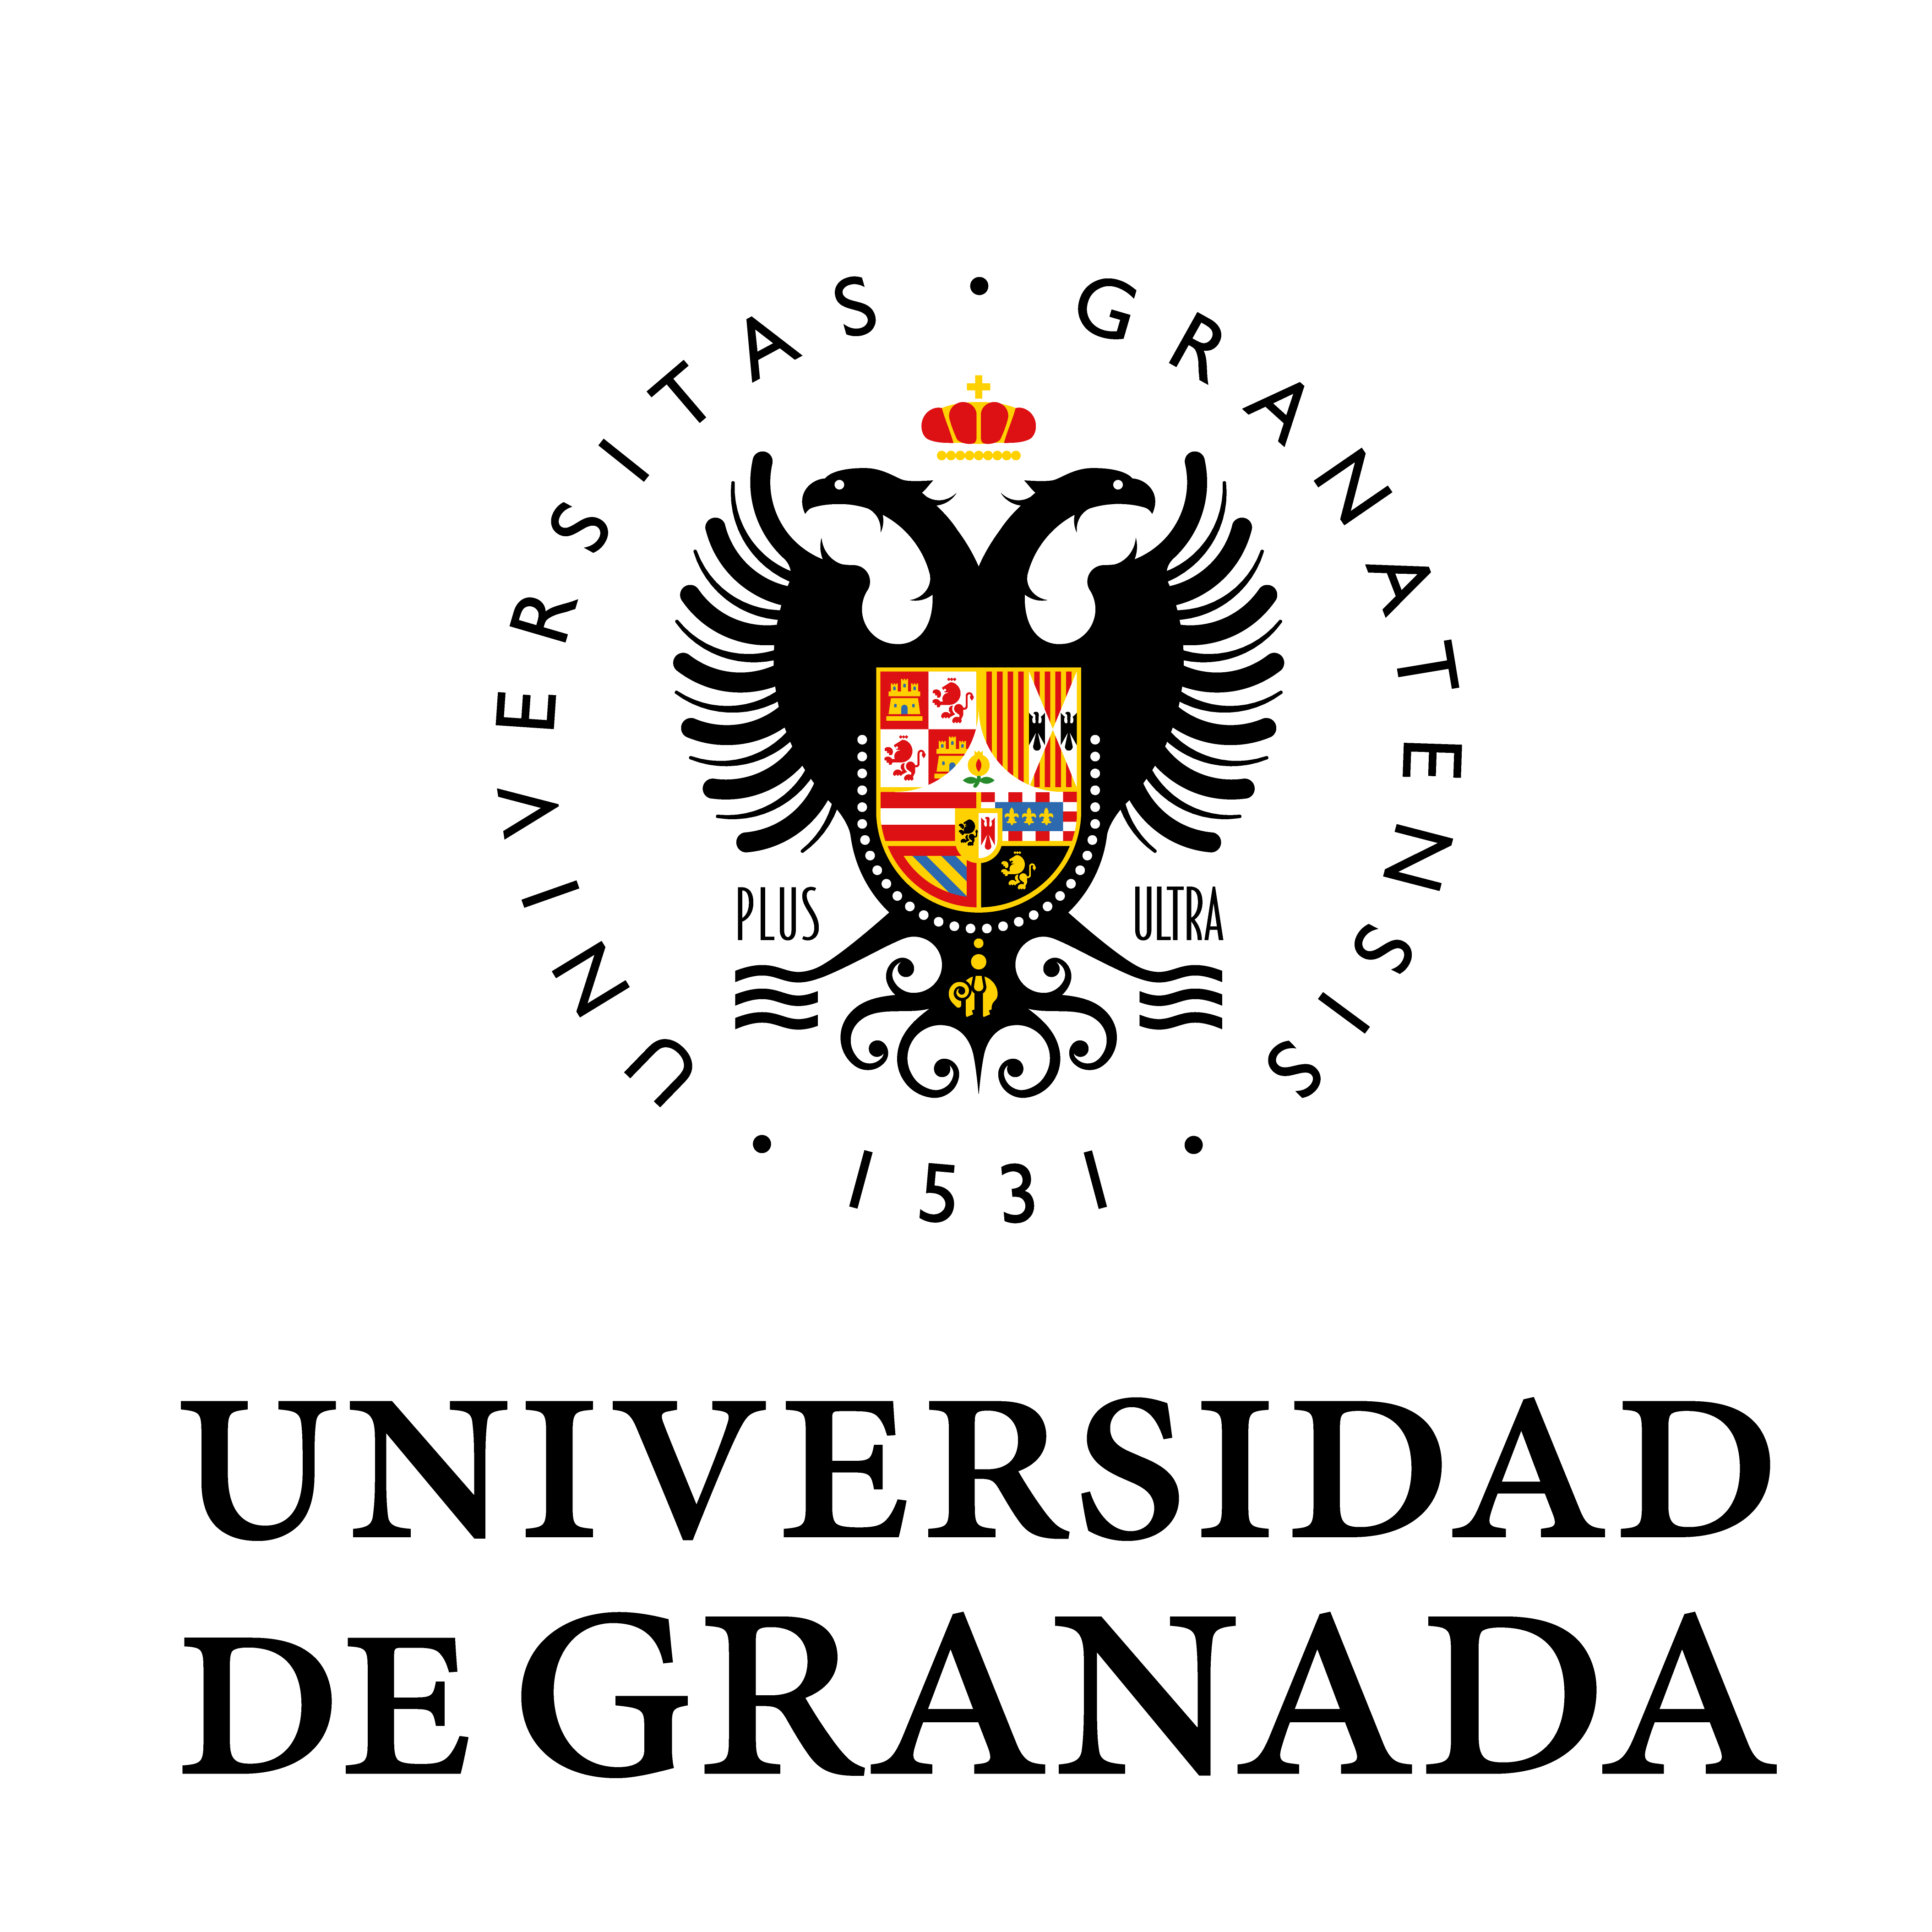
\includegraphics[width=0.5\textwidth]{images/logo-ugr.png}\par
    \vspace{1cm}
    {\Large\scshape Entornos Virtuales \par}
    {\huge\bfseries Texturas \par}
    \vspace{0.2cm}
    {\scshape Práctica 4 \par}
    \vfill
    {\large Víctor Vázquez Rodríguez  \par}
    {victorvazrod@correo.ugr.es \par}
    \vfill
    {\large Máster Universitario en Ingeniería Informática \par}
    \vspace{0.2cm}
    {Curso 2019/20 \par}
\end{titlepage}

En esta práctica, se han aplicado texturas al modelo que se ha ido definiendo en
las anteriores. En mi modelo de locomotora se aplican 4 texturas: acero, hierro
forjado, acero rojo y vidrio amarillo. Las texturas finales difieren ligeramente
de las establecidas en la práctica 2, pero los tonos son los mismos.

A la hora de aplicar las texturas y, para mantener la consistencia entre las
distintas mallas que las comparten, se han creado 4 materiales con sus
respectivas texturas que se han ido reutilizando para todo el modelo:

\begin{itemize}
    \item Acero: usado en los frenos, el centro de las ruedas y la palanca de la
          velocidad.
    \item Hierro forjado: todo el cuerpo de la locomotora, así como las ruedas y
          los faros.
    \item Acero rojo: Aplicado a la base de la locomotora.
    \item Rojo: Usando la misma textura del acero rojo, pero con menos reflejos,
          para el extremo de la palanca de la velocidad.
    \item Luz: Para los focos de los faros. Este material tiene más valor de la
          propiedad \textit{emit} que los demás.
\end{itemize}

\begin{figure}[h!]
    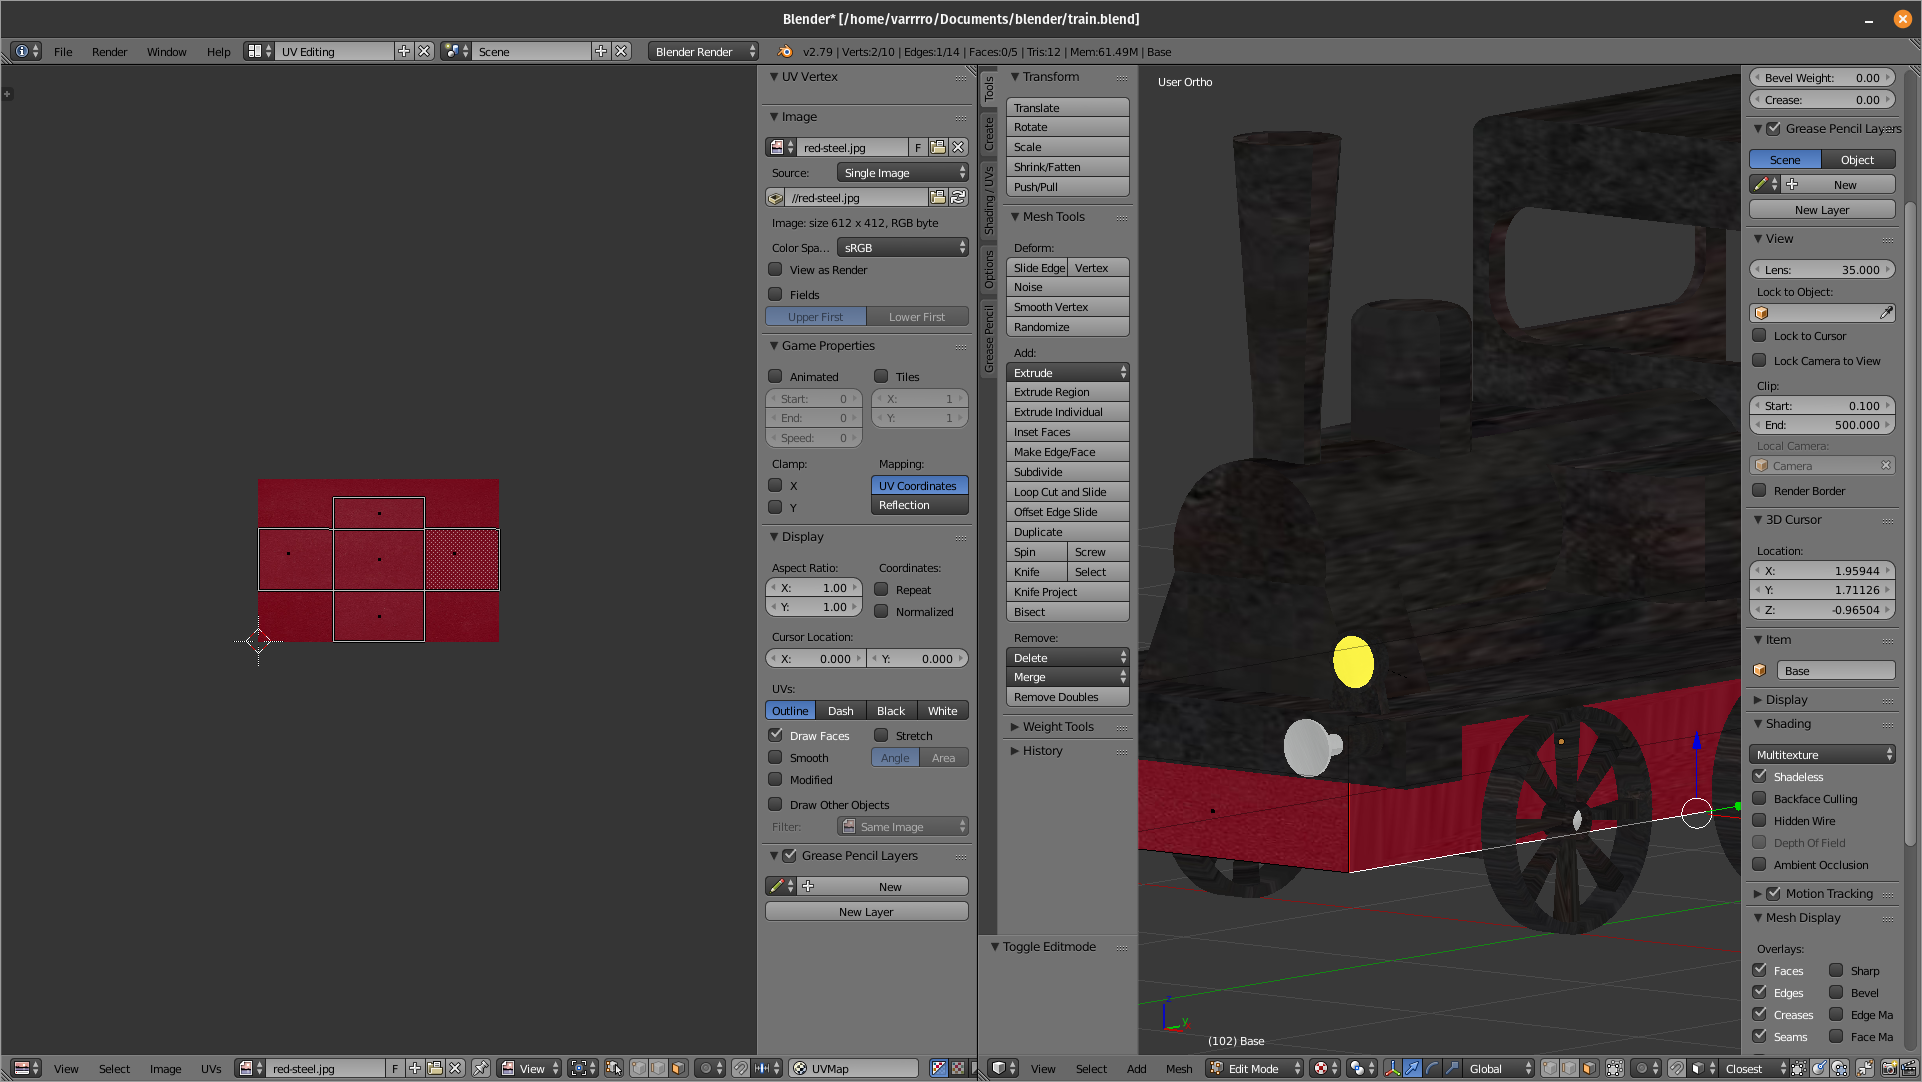
\includegraphics[width=\textwidth]{images/seams.png}
    \caption{\textit{Mapping} de la textura de la base de la locomotora usando costuras}
    \label{fig:seams}
\end{figure}

En algunos objetos había que aplicar más de una textura, como es el caso de los
faros y sus focos, o el cuerpo de la locomotora y su base. Por ello, se han
tenido que separar estos objetos en varias mallas para poder realizar los
\textit{mappings} de las texturas y aplicar los materiales por separado.

\begin{figure}
    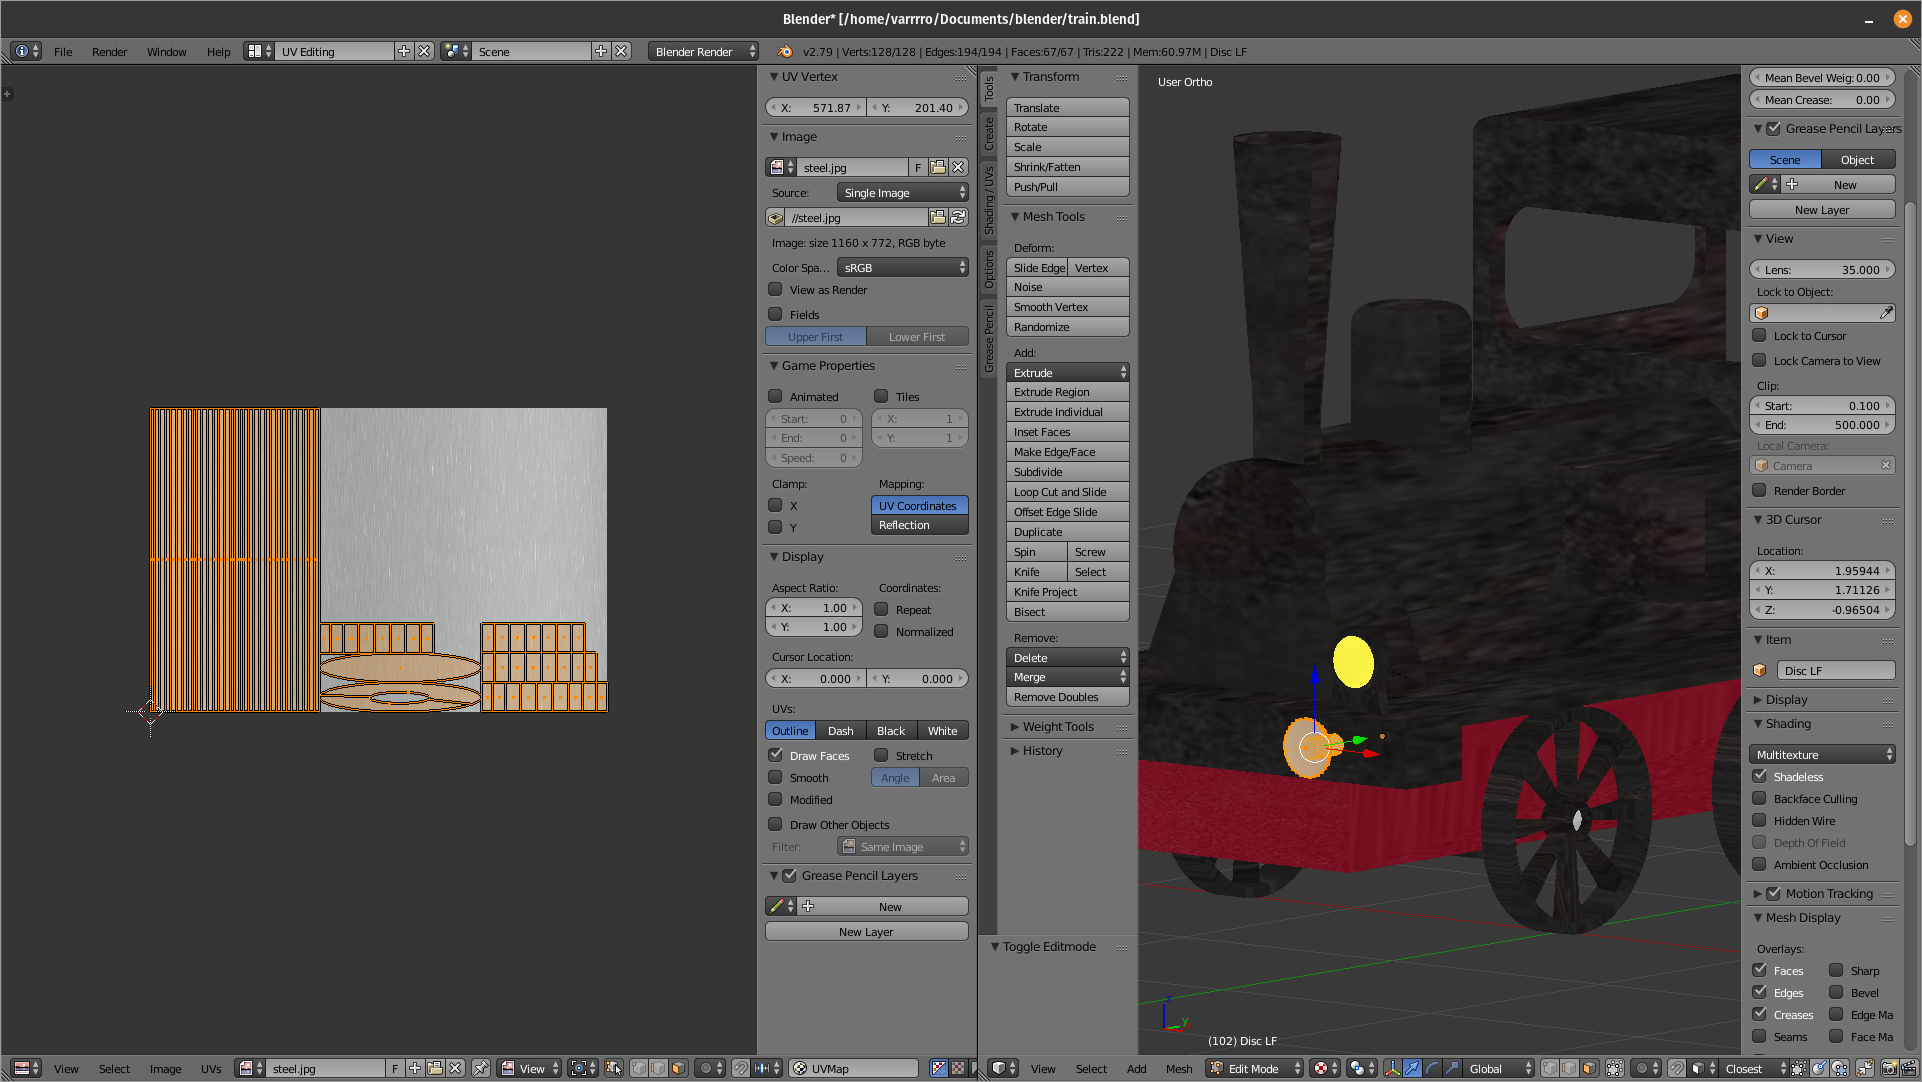
\includegraphics[width=\textwidth]{images/smart-uv.png}
    \caption{\textit{Mapping} de la textura de los frenos usando \textit{smart UV}}
    \label{fig:smart-uv}
\end{figure}

\begin{figure}
    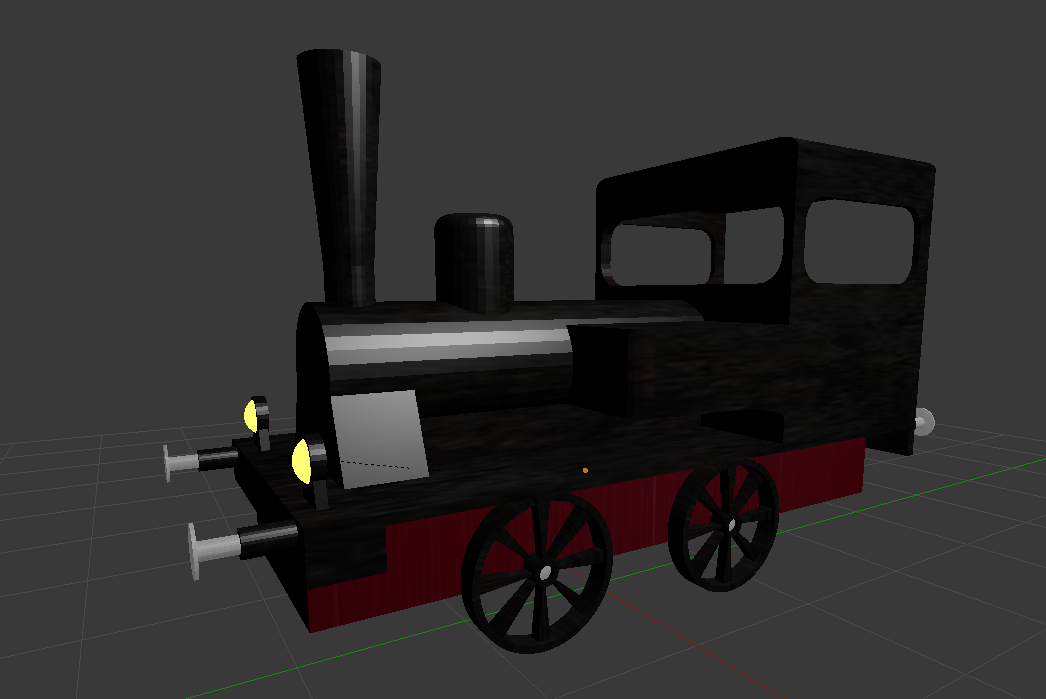
\includegraphics[width=\textwidth]{images/final.png}
    \caption{Modelo final tras la aplicación de los materiales y las texturas}
    \label{fig:final}
\end{figure}

Para crear los \textit{mappings} de las texturas a los objetos, en los objetos
más simples se ha hecho \textit{unwrap} directamente (esferas, cilindros) para
luego ir ajustándolos a la textura, mientras que en los objetos con formas más
complejas se ha usado la opción \textit{smart UV project} (figura
\ref{fig:smart-uv}). En algunos casos, como es el panel de control de la
locomotora o la base de ésta, se han marcado costuras (\textit{seams}) antes de
hacer el \textit{unwrap} (figura \ref{fig:seams}). El resultado final se puede
ver en la figura \ref{fig:final}.

\end{document}
